% Template for Cogsci submission with R Markdown

% Stuff changed from original Markdown PLOS Template
\documentclass[10pt, letterpaper]{article}

\usepackage{cogsci}
\usepackage{pslatex}
\usepackage{float}
\usepackage{caption}

% amsmath package, useful for mathematical formulas
\usepackage{amsmath}

% amssymb package, useful for mathematical symbols
\usepackage{amssymb}

% hyperref package, useful for hyperlinks
\usepackage{hyperref}

% graphicx package, useful for including eps and pdf graphics
% include graphics with the command \includegraphics
\usepackage{graphicx}

% Sweave(-like)
\usepackage{fancyvrb}
\DefineVerbatimEnvironment{Sinput}{Verbatim}{fontshape=sl}
\DefineVerbatimEnvironment{Soutput}{Verbatim}{}
\DefineVerbatimEnvironment{Scode}{Verbatim}{fontshape=sl}
\newenvironment{Schunk}{}{}
\DefineVerbatimEnvironment{Code}{Verbatim}{}
\DefineVerbatimEnvironment{CodeInput}{Verbatim}{fontshape=sl}
\DefineVerbatimEnvironment{CodeOutput}{Verbatim}{}
\newenvironment{CodeChunk}{}{}

% cite package, to clean up citations in the main text. Do not remove.
\usepackage{apacite}

% KM added 1/4/18 to allow control of blind submission


\usepackage{color}

% Use doublespacing - comment out for single spacing
%\usepackage{setspace}
%\doublespacing


% % Text layout
% \topmargin 0.0cm
% \oddsidemargin 0.5cm
% \evensidemargin 0.5cm
% \textwidth 16cm
% \textheight 21cm

\title{Consistency and variability in two children's home visual environment
across development}


\author{}

\begin{document}

\maketitle

\begin{abstract}
What do children tend to see in their everyday lives? While an
understanding of children's visual environment is central to both
theories of language acquisition and visual development, relatively
little work has examined the categories and objects that tend to be in
the infant view during everyday experience. Here, we analyzed the
prevalence of the superordinate categories (e.g., people, animals, food)
in the infant view in a longitudinal dataset of egocentric infant visual
experience (Sullivan et al., 2020). Overall, we found a surprising
amount of consistency in the broad characteristics of children's visual
environment across individuals and across developmental time, in
contrast to prior work examining the changing nature of the social
signals in the infant view. In addition, we analyzed the distribution
and identity of the categories that children tended to be touching or
interacting with in this data, confirming previous findings that these
objects tended to be distributed in a Zipfian manner (Clerkin et al.,
2017). Taken together, these findings take a first step towards
characterizing infants' changing visual environment, and call for future
work to examine the generalizability of these results and to link them
to learning outcomes.

\textbf{Keywords:}
Object categorization; infant visual experience; head-mounted cameras;
longitudinal data.
\end{abstract}

\hypertarget{introduction}{%
\section{Introduction}\label{introduction}}

What do children tend to see in their everyday lives? While an
understanding of children's visual environment is central to both
theories of language acquisition and visual development, we know
remarkably little about the categories and objects that tend to be in
the infant view, or in what format they are experienced. For example,
how often do infants tend to see animals in real-life vs.~in storybooks
or as toys? How consistent are the broad characteristics of children's
visual environments across individuals and across developmental time?

Over the past decade, researchers have begun to answer these questions
by documenting the infant egocentric perspective using head-mounted
cameras (Franchak, Kretch, Soska, \& Adolph, 2011; Yoshida \& Smith,
2008), quantifying the degree to which there are substantial shifts in
infants' viewpoints that may have downstream developmental
consequences.\\
Indeed, as adults it is hard to intuit how strange this viewpoint can
be, and how much it varies across development, transitioning over the
first two years of life from close-up views of faces to restricted views
of hands manipulating objects (Fausey, Jayaraman, \& Smith, 2016; Long,
Kachergis, Agrawal, \& Frank, 2020), with children's postural
developments to a large extent shaping what they see (Sanchez, Long,
Kraus, \& Frank, 2018). Most work, however, has focused on documenting
the social information that infants and children have access to across
early development (Fausey et al., 2016; Sanchez et al., 2018; Yoshida \&
Smith, 2008).

\begin{CodeChunk}
\begin{figure*}[h]

{\centering 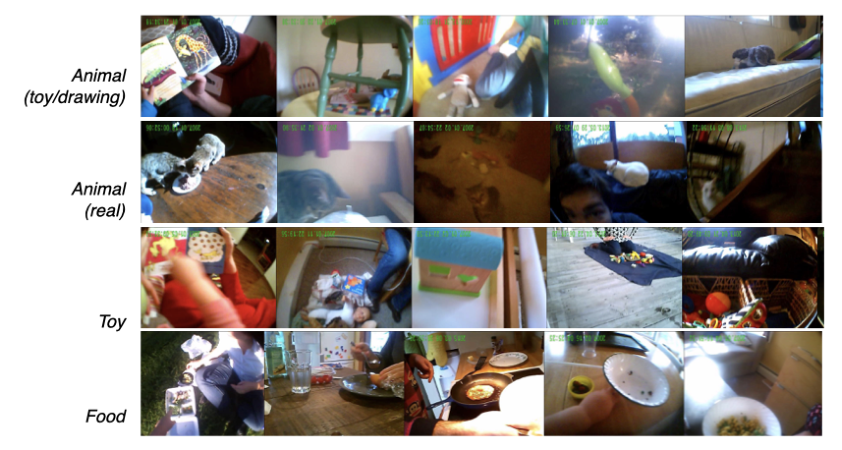
\includegraphics{figs/examples-1} 

}

\caption[Example frames with annotations of four different broad categories]{Example frames with annotations of four different broad categories.}\label{fig:examples}
\end{figure*}
\end{CodeChunk}

More recent research has made progress towards understanding what
objects tend to be the infant view, starting with annotating the
basic-level categories (e.g., spoons, cups) in the view of 8-month-olds
during mealtime. This research suggests that a small number of objects
are both pervasively present during mealtime and among infants'
first-learned words (Clerkin, Hart, Rehg, Yu, \& Smith, 2017), pointing
towards a link between visual experience and early word learning. These
findings suggest that a more complete understanding of the visual
environment of infants and young children could yield insights about the
inputs to both category learning and word learning.

Here, we take a step towards characterizing the visual environment of
young children by analyzing the categories of objects (e.g., animals,
vehicles, toys, people) present in the infant view in a longitudinal
corpus of head-mounted camera data (Sullivan, Mei, Perfors, Wojcik, \&
Frank, 2020). To start, we choose to annotate these broad categories --
rather than the basic-level identities of all objects that were present
-- as these less detailed annotations allow us to collect data about
many more frames from the dataset. We thus collected human annotations
of a randomly sampled set of 24,000 frames from two children in the
longitudinal dataset, allowing the analysis of the proportion of broad
categories in the infant view from 6-32 months of age. To complement
this broad sample, we hand-annotated the basic-level categories of the
objects that children were interacting with in the subset of frames
where children's hands were visible (3000 frames), providing a closer
look into the kinds of objects children have the most intensive visual
and haptic experience with.

Using these annotations, we conducted four sets of analyses. First,
using the broad category annotations, we examined whether the proportion
of animals vs.~inanimate objects would be relatively equal in the infant
view. A long literature has documented that even newborns have a
tendency to attend to animate agents (Farroni et al., 2005), and visual
cortex dedicates a remarkable amount of space to processing animals
(Konkle \& Caramazza, 2013). Furthermore, animal words tend to be among
children's first-learned words (Frank, Braginsky, Yurovsky, \& Marchman,
n.d.). However, at present, it is unknown whether (non-human) animates
(e.g., cats, dogs, other animals) are prevalent in the infant viewpoint,
and whether they tend to be exemplars of real-life animals (e.g., ducks
at a park, pet dogs) or mostly illustrations in storybooks or as toy
stuffed animals. Second, we examined the co-occurrence between these
broad object categories across visual scenes. While some activity
contexts (e.g., storytime) and lead to intuitive co-occurrences between
object categories (e.g., between books and people), not all activities
are intuitive or consistent. We conducted a set of data-driven,
exploratory analyses of the co-occurrence statistics of these broad
categories to identify other, reliable patterns in how infants
experience their visual world. Third, prior work documenting the
proportion of faces/hands in view has suggested some developmental
changes in how children experience their visual across this same age
range--including in this same dataset (Long et al., 2020). Thus, one
possibility is that as children learn to crawl and walk on their own
(Franchak et al., 2011; Long et al., 2020; Sanchez et al., 2018), some
categories that children are likely to interact with (i.e., toys, small
objects) could become more prevalent in the child's view across age,
whereas other, more stable categories (i.e., furniture) might show
relative consistency. On the other hand, the broad characteristics
children's visual environments may be relatively stable andmostly
determined by the activities that they tend to engage in. We thus
examined this hypothesis by exploring the prevalence of each of the
broad categories that were annotated across developmental time and
across both children. Finally, we examined the basic-level annotations
of the categories that children tended to interact with, evaluating the
degree to which these objects tend to be distributed in a Zipfian manner
(and thus the generality of Clerkin et al., 2017).

\begin{CodeChunk}
\begin{figure*}[h]

{\centering 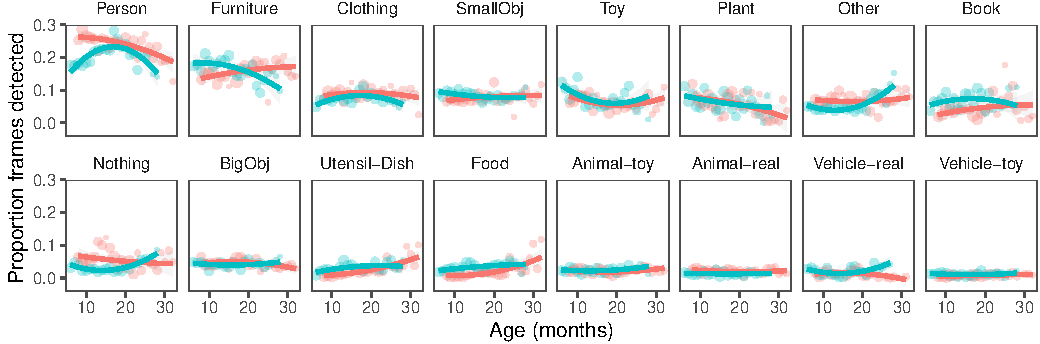
\includegraphics{figs/freq_by_category-1} 

}

\caption[Frequency of categories annotated across the 24K random frames plotted as a function of each child's age (in months)]{Frequency of categories annotated across the 24K random frames plotted as a function of each child's age (in months).}\label{fig:freq_by_category}
\end{figure*}
\end{CodeChunk}

\hypertarget{method}{%
\section{Method}\label{method}}

\hypertarget{dataset}{%
\subsection{Dataset}\label{dataset}}

The dataset is described in detail in Sullivan et al. (2020). Children
wore Veho Muvi miniature cameras mounted on a custom camping headlamp
harness (``headcams'') at least twice weekly, for approximately one hour
per recording session. One weekly session was on the same day each week
at a roughly constant time of day, while the other(s) were chosen
arbitrarily at the participating family's discretion. At the time of the
recording, all three children were in single-child households. Videos
captured by the headcam were 640x480 pixels, and a fisheye lens was
attached to the camera to increase the field of view to approximately
109 degrees horizontal x 70 degrees vertical. We randomly sampled 24000
frames from videos of two of the children in the dataset (S, A) over the
entire age range.

\hypertarget{annotation-procedures}{%
\subsection{Annotation procedures}\label{annotation-procedures}}

\hypertarget{broad-categories-in-view}{%
\subsubsection{Broad categories in
view}\label{broad-categories-in-view}}

Annotations of the broad categories in the dataset were obtained using
AWS Sagemaker annotations using credits from {[}blinded{]}. Participants
were instructed to select all of the categories that could be applied to
an image; two workers annotated each image, and each category that was
annotated for an image was assigned a confidence score (possible range:
0-1, range in dataset: .5-1). Participants selected whether the
following categories were present in the shown image: Animal (real),
Animal (toy/drawing), Vehicle (real), Vehicle (toy/drawing), Plant,
Clothing, Person, Furniture, Food, Utensil/Dish, Other Small Object,
Other Big Object, Book, Other, or Nothing visible. We included ``other
small objects'' and ``other big objects'' as categories that
participants could use to indicate objects that fell outside of these
traditional superordinate categories (i.e.~furniture, plant, toy).
Additional instructions were provided to specify that `other big object"
refers to an object that is bigger than a chair, and that 'other small
object' refers to an object that is small enough to be held with one or
two hands (Konkle \& Oliva, 2012). Annotators were required to select at
least one category before proceeding. Individual annotations had
confidence scores below the 25\%th percentile were excluded from
analyses (although all conclusions hold with and without these
low-confidence annotaitons). Each child's age was calculated in days
relative to the date that the videos were filmed and converted to
months.

\hypertarget{objects-in-the-childs-reach}{%
\subsubsection{Objects in the child's
reach}\label{objects-in-the-childs-reach}}

We also annotated the objects that children were interacting with in a
subset of these frames. Specifically, we selected the frames in which a
previous set of participants recruited via Amazon Mechanical Turk
annotated whether the hands present in a given image belong to an adult
or a child and drew bounding boxes around those hands; these frames a
subset of frames that were previously annotated by another set
participants who indicated that a hand was present. This resulted in a
set of 3050 images that were then annotated by the authors who
established labeling conventions prior to annotation. Annotators noted
what object the child was interacting with in frames containing
children's hands, using basic level object categories, such as ``bird''
and ``cracker.'' When children were interacting with drawing or toy
versions, these annotations were marked a `-drawing' and `-toy'
modifier. If a view was allocentric or there were no child hands in
view, these frames were excluded from analysis. Finally, if there was no
object or the object was unclear, these frames were marked accordingly.

\hypertarget{results}{%
\section{Results}\label{results}}

\hypertarget{which-categories-are-prevalent-in-the-childs-view}{%
\subsection{Which categories are prevalent in the child's
view?}\label{which-categories-are-prevalent-in-the-childs-view}}

First, we examined the overall prevalence of each broad category in the
infant view. Somewhat surprisingly, we found that the prevalence of most
of these categories were relatively stable both across the two children
in the dataset as well as over developmental time. This stands in
contrast to prior work on the prevalence of faces/hands in the infant
view (Fausey et al., 2016; Long et al., 2020), suggesting that these
broader characteristics of children's visual experience may be more
consistent.

\begin{CodeChunk}
\begin{figure*}[h]

{\centering 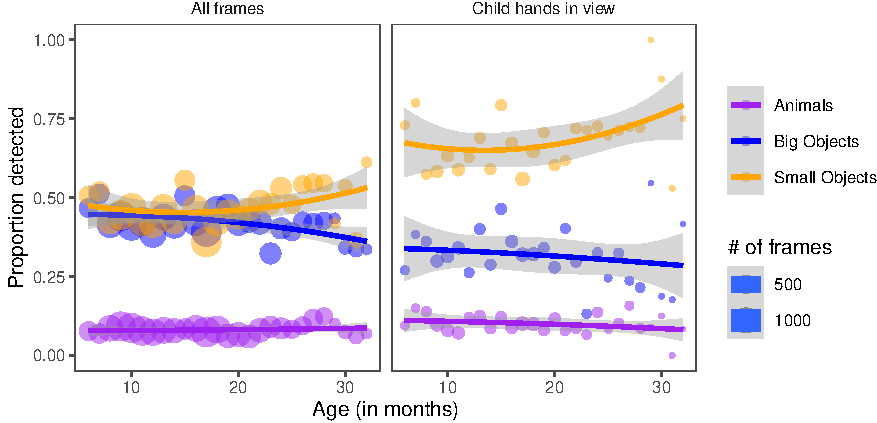
\includegraphics{figs/anim_size-1} 

}

\caption[Frequency of animals (including toys) relative to big and small inanimate objects detected in the dataset, both when analyzing all frames that were annotated (left) and the subset of frames where a child's hand was visible in the frame (right)]{Frequency of animals (including toys) relative to big and small inanimate objects detected in the dataset, both when analyzing all frames that were annotated (left) and the subset of frames where a child's hand was visible in the frame (right).}\label{fig:anim_size}
\end{figure*}
\end{CodeChunk}

We next examined the details of these environments. We found that people
were by far the most prevalent of these categories: over 20\%~of the
frames that were annotated contained people, far more than any
categories (including all kinds of toys combined). In contrast, there
were relatively few instances of animals in the infant view--either as
toys or their real life counterparts. Less than 5\%~of these frames that
contained any kind of depicted or real animal, and depicted vs.~real
animals were present in equal proportion. Manual inspection of these
frames containing animals revealed that the ``real'' animals had
relatively little variety -- they were overwhelmingly frames containing
images of household pets (i.e., cats, dogs, and chickens, in the case of
A), whereas the animals that were ``toys/drawings'' depicted a much
larger variety of animals, as one might expect. Overall, these results
suggest that -- at least for these children -- people are much more
frequent that depictions or real-life versions of animals, indicating
that toys and drawings may provide frequent input to their
representations of these categories -- despite the fact that animal
names are often among children's first words (Frank et al., n.d.) and
often referenced in storybooks.

Far more prevalent than animals, instead, were objects. Views of
furniture were the next most common category after ``people''. However,
in older age ranges, ``big objects'' -- including furniture, vehicles,
and other big objects -- tended to be less frequently in the view of
infants than ``small'' objects -- including toys (of all kinds), food,
utensils, books, and other small objects (see Figure
\ref{fig:anim_size}). This effect was much exaggerated when we conducted
this analysis on a subset of the frames where children's hands were also
in view -- as a proxy for times when children were interacting with
objects. In these frames, small objects tended to be much more prevalent
in the frames that we annotated. These data are consistent with the idea
that as children grow and become more adept at handling objects on their
own, small objects may tend to be more often in view.

\hypertarget{which-categories-co-occur-in-childrens-visual-environment}{%
\subsection{Which categories co-occur in children's visual
environment?}\label{which-categories-co-occur-in-childrens-visual-environment}}

Next, we next examined the degree to which these broad categories
appeared together in different frames. Figure \ref{fig:coocc_stats}
shows the co-occurrence of the broad categories, and reveals some
relatively intuitive patterns that may reflect activity contexts. For
example, ``dishes'' and ``food'' co-occured quite frequently together,
as did ``people'' and ``clothing,'' and most animals that were toys or
drawings appeared when ``books'' were also present. Broadly, these
results suggest that activity contexts -- such as playtime, mealtime, or
storytime -- may have a considerable influence on the categories that
tend to be in the infant view, pointing towards the role of these
structured activity contexts for shaping what children learn about these
categories (Bruner, 1985).

\begin{CodeChunk}
\begin{figure}[h]

{\centering 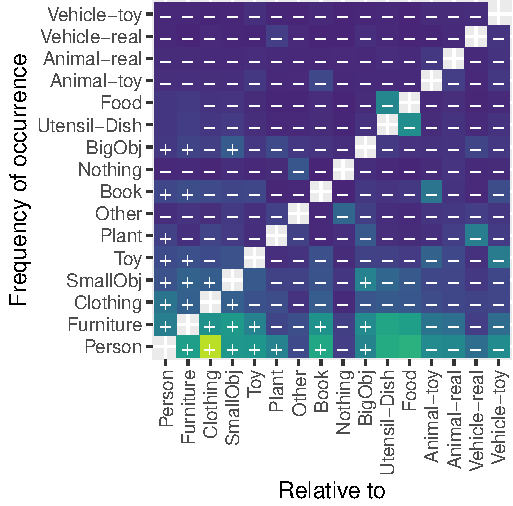
\includegraphics{figs/coocc_stats-1} 

}

\caption[Co-ccurance between different categories detected in the dataset across all frames]{Co-ccurance between different categories detected in the dataset across all frames.  Each cell represents the probability that the category the y-axis (e.g., clothing) occurs relative to the occurance of the category on the x-axis (e.g., person). Lighter values indicate higher probabilities of co-occurance (max=.8, min=0).}\label{fig:coocc_stats}
\end{figure}
\end{CodeChunk}

\hypertarget{which-objects-do-children-tend-to-interact-with}{%
\subsection{Which objects do children tend to interact
with?}\label{which-objects-do-children-tend-to-interact-with}}

While many different categories may be in the child's view, not all of
these objects may be equally important in the child's immediate
environment. In particular, objects that children physically interact
with may be more likely to be those that they form robust
representations of, and by extension those whose labels are learned
earlier. In this analysis, we sought to analyze the basic-level
identities of the objects that children interacted with in their home
environments -- and the distributions of those object categories. While
some work has suggestion that the objects in the infant view tend to
have a Zipfian distribution (Clerkin et al., 2017), it is unclear
whether this only applies to the objects that tend to be in view during
mealtime vs.~the objects that children tend to actually interact with
during a wide range of activities.

We found that the distribution of the objects in view roughly followed a
power law distribution (Clerkin et al., 2017), confirming that the
distribution of the objects that children both see and interact are
likely to be skewed. When we examined which categories were most
frequent, we found that books were overwhelming the most present object
in the views of these two children, comprising over 20\% of the objects
that children's hands were interacting with. Generic toys (that were
unidentifiable to the authors as specific toys) were the next most
frequent object category, and children were often seen to be touching or
holding on to their caregivers (see top 20 most frequent categories in
Figure \ref{fig:freq_interact}). We also saw evidence of some coarse
developmental differences, attesting to different play habits across
childhood: for example, when these children were older than 18 months
they were often seen holding crayons or paper, this was untrue in the
views capture during their early infancy (i.e.~6-12 months of age).

\begin{CodeChunk}
\begin{figure}[h]

{\centering 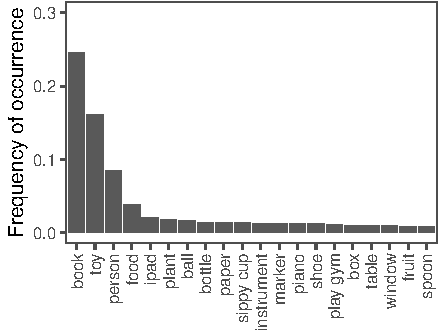
\includegraphics{figs/freq_interact-1} 

}

\caption[Top 20 most frequent categories that children's hands were interacting with in these egocentric videos]{Top 20 most frequent categories that children's hands were interacting with in these egocentric videos.}\label{fig:freq_interact}
\end{figure}
\end{CodeChunk}

\hypertarget{general-discussion}{%
\section{General Discussion}\label{general-discussion}}

Here, we analyzed the consitency and variablity of the categories and
the objects in the infant view, examining a sample of random frames
taken from a longitudinal dataset of two children (Sullivan et al.,
2020). Overall, we found relative consistency in child's visual
environment over development, contrary to prior work on the prevalence
of social signals over this same developmental time period (Fausey et
al., 2016; Long et al., 2020). The relative proportions of broad
categories of objects (i.e., furniture, toys, animals, people) was
relatively consistent between the two individuals and across
developmental time. People were most frequent, yet a non-trivial
proportion of frames didn't contain any discernible objects at all.
Data-driven analysis of these category co-occurrence revealed relatively
stereotypical combinations (i.e.~utensils and food, people and
clothing), suggesting that these activities may structure the objects in
the infant view to some extent. While the proportion of small objects in
view did seem to show somewhat of a u-shape curved around the first
birthday -- consistent with the hypothesis that children may see fewer
toys as they are learning to crawl and walk (Long et al., 2020) -- this
remains to be confirmed with future research. Instead, postural
developments and cognitive milestones may lead to finer-grain changes in
how children view objects or the diversity of exemplars that tend to be
view.

However, while people were incredibly frequent in the child's view,
animals -- either as toys or their real-life versions -- were relatively
infrequent and occurred in equal proportions. Instead, the child's view
was most likely to be dominated by small objects that they interact with
-- such as food, books, or toys. We also found that the proportion of
these small objects increased dramatically when we restricted our
analysis to frames where the child's hands are in view, suggesting that
the statistics of children's visual environment shift substantially when
they are acting on the world themselves (i.e., while playing). Further,
given that animal words are among children's first-learned words, these
results underscore that children's heightened attention to animals
(Farroni et al., 2005) likely interacts with frequency of occurrence in
the visual field to drive early category learning.

Finally, we examined the categories that children tend to interact with
in these egocentric videos, finding that these children were often
manipulating books and, more generally, that the distribution of these
objects seem to follow a Zipfian distrition. Indeed, as mealtime has
previously been used to characterize the objects in the infant view
(Clerkin et al., 2017) and frames with food or utensil and dishes
accounted for less than 5\%~of view, we were unsure whether this would
be the case. However, this analysis suggests that -- at least in this
sample -- that infants may more generally interact with different object
categories in a relatively Zipfian manner.

Overall, this work takes a first step in characterizing the categories
in visual environment of children over development, calling for future
work to understand the generalizability of these findings beyond the
present dataset. While we found relatively consistent results across
both age and the two children in the dataset, both of these children are
from relatively similar households and cultural contexts. Nonetheless,
we predict that the broad characteristics of these environments may be
likely to generalize to many other contexts. In particla, we predict
that most children in urban or surburban contexts are unlikely to see
real animals more frequently than depicted animals, and the distribution
of objects that children interact with are likely to follow a Zipfian
distribution -- regardless of which specific objects these are.

More broadly, this work highlights the need for systematic
investigations of how the frequency of the categories in the child's
view interacts with different attentional biases, learning mechanisms,
and social cues to produce robust representations that support category
and early language learning. An understanding of what is -- and what is
not -- learnable solely from frequent exposures will provide constraints
on our accounts of the learning mechanisms that allow children to learn
so much about their visual world so quickly.

\hypertarget{acknowledgements}{%
\section{Acknowledgements}\label{acknowledgements}}

(Blinded)

\hypertarget{references}{%
\section{References}\label{references}}

\setlength{\parindent}{-0.1in} 
\setlength{\leftskip}{0.125in}

\noindent

\hypertarget{refs}{}
\leavevmode\hypertarget{ref-bruner1985role}{}%
Bruner, J. (1985). The role of interaction formats in language
acquisition. In \emph{Language and social situations} (pp. 31--46).
Springer.

\leavevmode\hypertarget{ref-clerkin2017}{}%
Clerkin, E. M., Hart, E., Rehg, J. M., Yu, C., \& Smith, L. B. (2017).
Real-world visual statistics and infants' first-learned object names.
\emph{Phil. Trans. R. Soc. B}, \emph{372}(1711), 20160055.

\leavevmode\hypertarget{ref-farroni2005newborns}{}%
Farroni, T., Johnson, M. H., Menon, E., Zulian, L., Faraguna, D., \&
Csibra, G. (2005). Newborns' preference for face-relevant stimuli:
Effects of contrast polarity. \emph{Proceedings of the National Academy
of Sciences}, \emph{102}(47), 17245--17250.

\leavevmode\hypertarget{ref-fausey2016}{}%
Fausey, C. M., Jayaraman, S., \& Smith, L. B. (2016). From faces to
hands: Changing visual input in the first two years. \emph{Cognition},
\emph{152}, 101--107.

\leavevmode\hypertarget{ref-franchak2011}{}%
Franchak, J. M., Kretch, K. S., Soska, K. C., \& Adolph, K. E. (2011).
Head-mounted eye tracking: A new method to describe infant looking.
\emph{Child Development}, \emph{82}(6), 1738--1750.

\leavevmode\hypertarget{ref-frank2020}{}%
Frank, M. C., Braginsky, M., Yurovsky, D., \& Marchman, V. A. (n.d.).
\emph{Variability and Consistency in Early Language Learning: The
Wordbank Project}. Cambridge, MA: MIT Press. Retrieved from
\url{http://wordbank-book.stanford.edu}

\leavevmode\hypertarget{ref-konkle2013tripartite}{}%
Konkle, T., \& Caramazza, A. (2013). Tripartite organization of the
ventral stream by animacy and object size. \emph{Journal of
Neuroscience}, \emph{33}(25), 10235--10242.

\leavevmode\hypertarget{ref-konkle2012familiar}{}%
Konkle, T., \& Oliva, A. (2012). A familiar-size stroop effect:
Real-world size is an automatic property of object representation.
\emph{Journal of Experimental Psychology: Human Perception and
Performance}, \emph{38}(3), 561.

\leavevmode\hypertarget{ref-long2020}{}%
Long, B., Kachergis, G., Agrawal, K., \& Frank, M. C. (2020). Detecting
social information in a dense database of infants' natural visual
experience. \emph{Https://Psyarxiv.com/Z7tdg/}.

\leavevmode\hypertarget{ref-sanchez2018postural}{}%
Sanchez, A., Long, B., Kraus, A. M., \& Frank, M. C. (2018). Postural
developments modulate children's visual access to social information. In
\emph{Proceedings of the 40th annual conference of the cognitive science
society}.

\leavevmode\hypertarget{ref-SAYcam}{}%
Sullivan, J., Mei, M., Perfors, A., Wojcik, E., \& Frank, M. C. (2020).
SAYCam: A large, longitudinal audiovisual dataset recorded from the
infants perspective. \emph{PsyArXiv}. Retrieved from
\url{https://psyarxiv.com/fy8zx/}

\leavevmode\hypertarget{ref-yoshida2008}{}%
Yoshida, H., \& Smith, L. B. (2008). What's in view for toddlers? Using
a head camera to study visual experience. \emph{Infancy}, \emph{13}(3),
229--248.

\bibliographystyle{apacite}


\end{document}
